\documentclass[english,serif,mathserif,xcolor=pdftex,dvipsnames,table]{beamer}
\usepackage{gc3}

\title[VM-MAD]{%
  Cloudbursting computational clusters
}

\author[R.~Murri]{Riccardo Murri \\ \texttt{<riccardo.murri@uzh.ch>}}
\institute[GC3, Univ. of Zurich]{% will appear on the bottom line
  \href{http://www.gc3.uzh.ch/}{GC3: Grid Computing Competence Center},
  \\
  \href{http://www.uzh.ch/}{University of Zurich}
}
\date{Nov.~29, 2012} 

% see: http://tex.stackexchange.com/questions/51113/horizontal-equivalent-to-raisebox
\newcommand{\shiftleft}[2]{\makebox[0pt][r]{\makebox[#1][l]{#2}}}
\newcommand{\shiftright}[2]{\makebox[#1][r]{\makebox[0pt][l]{#2}}}
       
\begin{document}

\maketitle


\begin{frame}
  \frametitle{VM-MAD / 1}
  \begin{center}
    \textbf{V}irtual \textbf{M}achines \textbf{M}anagement 
    \\ and \textbf{A}dvanced \textbf{D}eployment

    \+
    Joint project of ETH, UZH, FGCZ, SWITCH \\ funded under the AAA/SWITCH scheme

    \+ 
    \emph{
      ``Provide simple mechanisms to deploy complex scientific
      applications on heterogeneous hardware and software resources
      using virtualization techniques.''
    }
  \end{center}
\end{frame}


\begin{frame}
  \frametitle{VM-MAD / 2}
  \begin{center}
    {\em Minimal impact on current usage patterns}

    \+ Progressive migration \\ from classic ``HPC cluster in the basement'' model \\ towards virtualized infrastructures

    \+ {\em Cloudbursting}

    \+ Integration with the SMSCG \\ national grid infrastructure 
  \end{center}
\end{frame}


\begin{frame}
  \frametitle{Example use case: Drosophila proteome}
  \begin{columns}
    \begin{column}{.30\textwidth}
      % Frequency vs Number of Tandem MS per run
      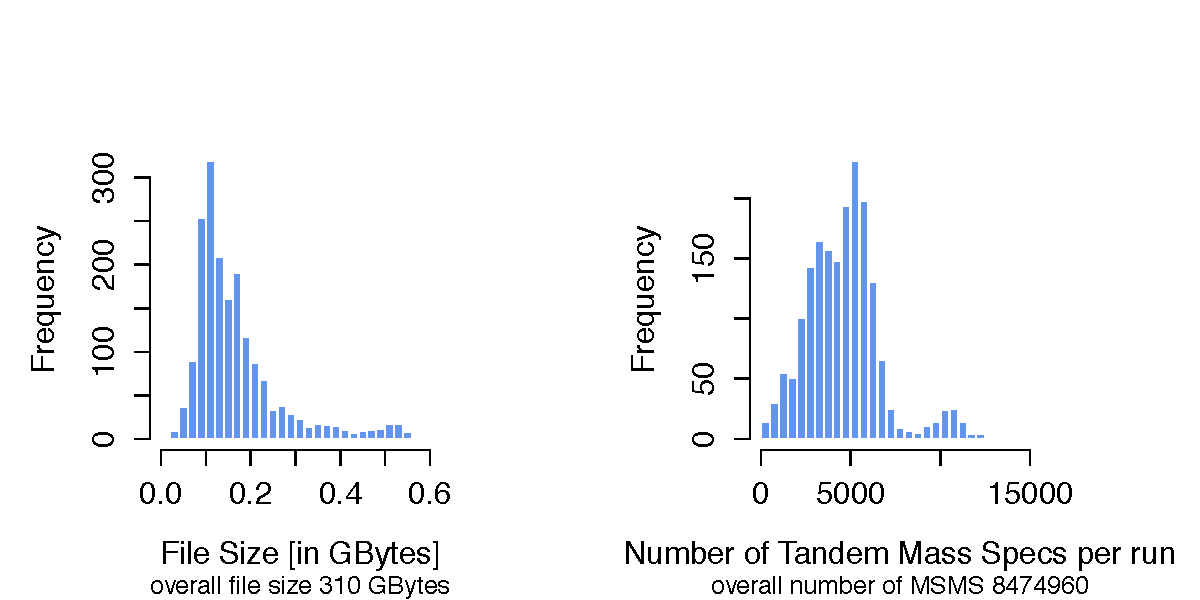
\includegraphics[viewport=10.0cm 0.0cm 20.0cm 10.0cm, clip, height=\columnwidth]{fig/ms}
      \\
      % Frequency vs File Size graph
      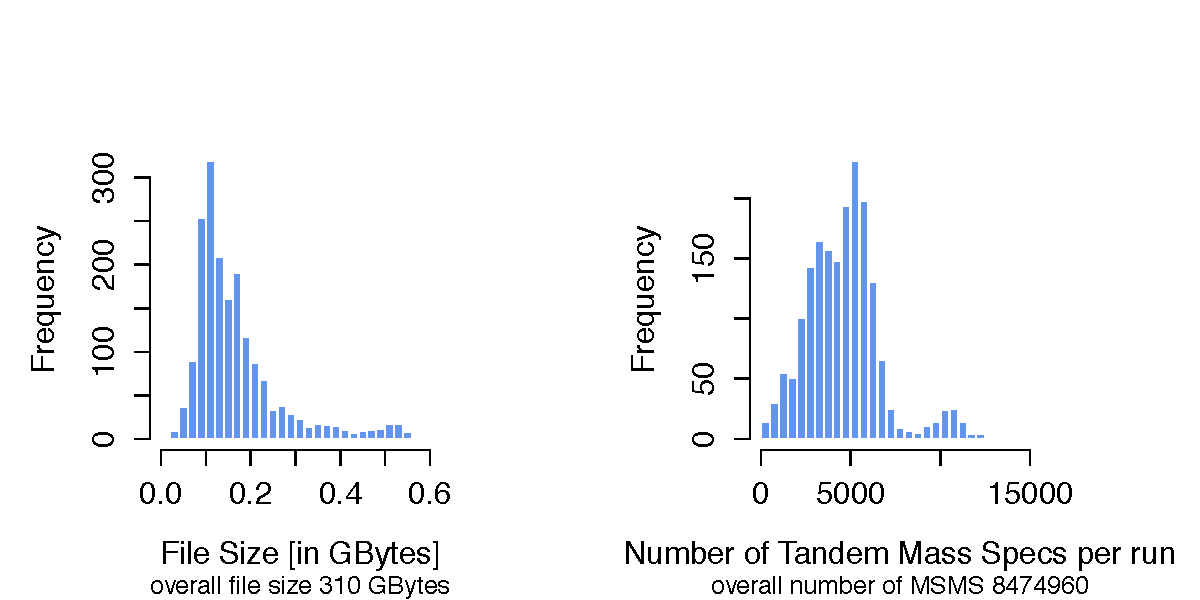
\includegraphics[viewport=0.0cm 0.0cm 10.0cm 10.0cm, clip, height=\columnwidth]{fig/ms}
    \end{column}
    \begin{column}{.75\textwidth}
      Some numbers from the ``bio'' side:
        \begin{itemize}
        \scriptsize
        \item 1'800 (LC)-MS/MS runs
        \item $\pm 3$Da peptide mass tolerance
        \item $\approx$ 10'000 peptides in the MS window
        \item 8'474'960 MS/MS
        \end{itemize}
        \begin{references}
          Nature Biotechnology 25, 576--583 (2007).
        \end{references}

        \+
        On the ``IT'' side:
        \begin{itemize}
        \scriptsize
        \item Many \emph{independent} single-thread jobs
        \item Perfect match for a batch-computing cluster!
        \item But local compute cluster already quite busy\ldots
        \end{itemize}
    \end{column}
  \end{columns}
\end{frame}

% LONG VERSION: (needs to be checked by CP)
%
% \begin{frame}
%   \frametitle{Example use case: Drosophila proteome / 1}
%   Combined lab and computational effort:
%   \begin{enumerate}[\color{gray}\em 1.]
%   \item Prepare peptide samples and run them through the Mass Spectrometer
%   \item For each peptide sample, run two MS measurements:
%     \begin{enumerate}[\em A.]
%     \item\label{m1} Measure the mass of the peptide ($\pm$ tolerance)
%     \item\label{m2} Fragment the sample into constituent aminoacids, then measure the MS spectrum of this ``aminoacid fragment ion soup''
%     \end{enumerate}
%   \item By~{\em \ref{m1}.} we know the candidate peptides
%   \item \alert<2>{Match them to the actual fragment ion spectra
%       computed in~{\em \ref{m2}.}}
%   \end{enumerate}

%   \+
%   \visible<2>{
%     This is the computationally intensive part!
%   }
% \end{frame}


% \begin{frame}
%   \frametitle{Example use case: Drosophila proteome / 2}
%   \begin{columns}
%     \begin{column}{.30\textwidth}
%       % Frequency vs Number of Tandem MS per run
%       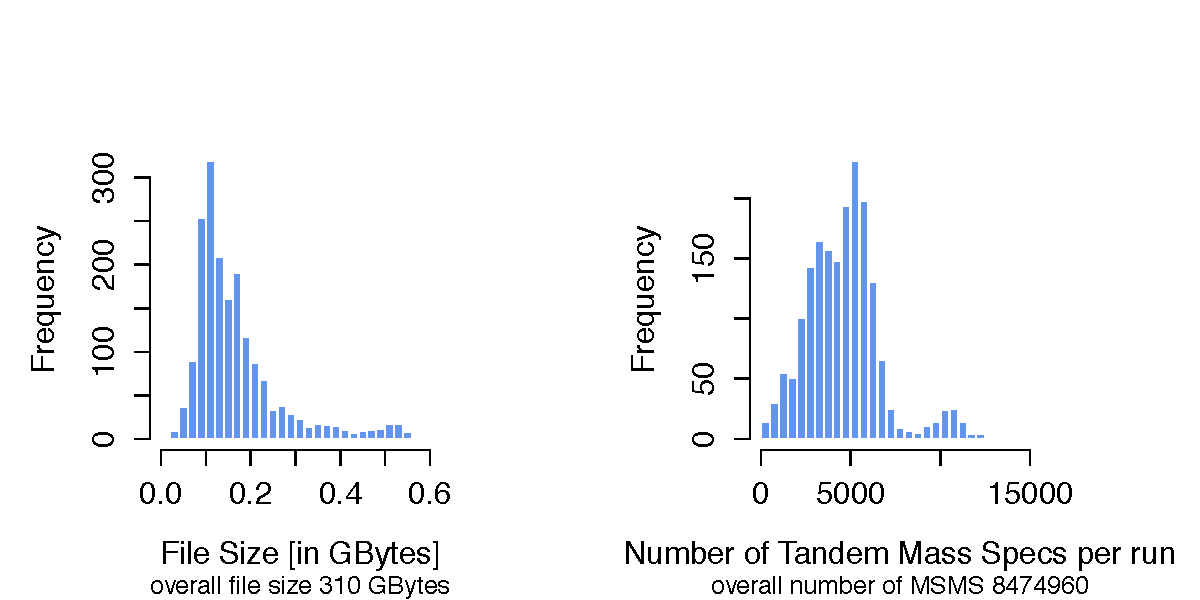
\includegraphics[viewport=10.0cm 0.0cm 20.0cm 10.0cm, clip, height=\columnwidth]{fig/ms}
%       \\
%       % Frequency vs File Size graph
%       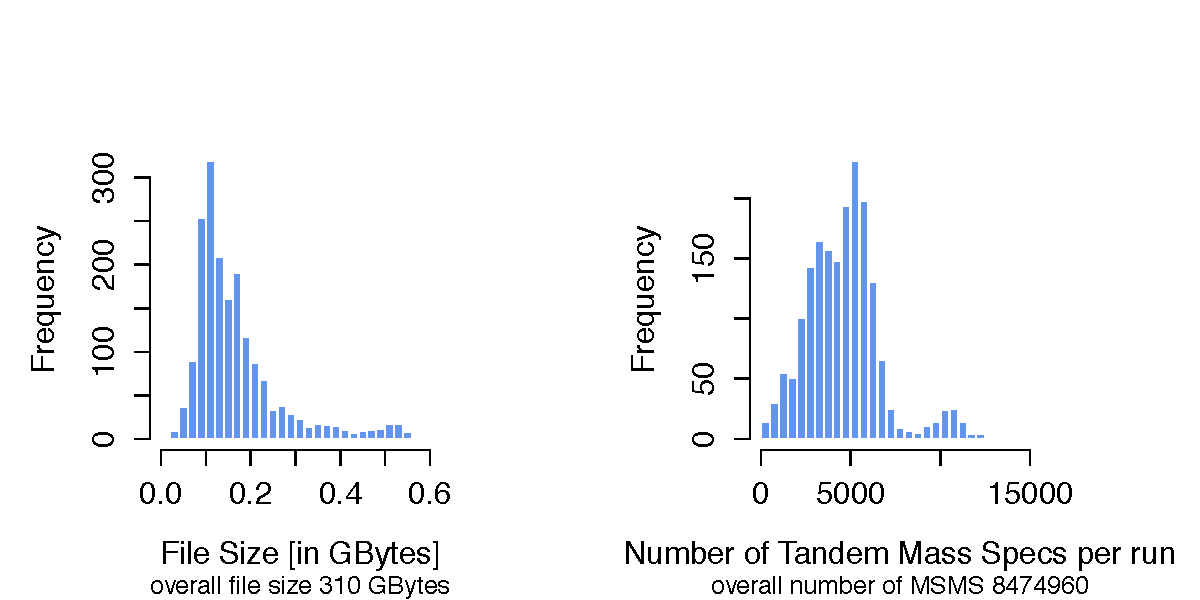
\includegraphics[viewport=0.0cm 0.0cm 10.0cm 10.0cm, clip, height=\columnwidth]{fig/ms}
%     \end{column}
%     \begin{column}{.75\textwidth}
%       Some Numbers:
%         \scriptsize
%         \begin{itemize}
%         \item 1'800 (LC)-MS/MS runs
%         \item $\pm 3$Da peptide mass tolerance
%         \item $\approx$ 10'000 peptides in the MS window
%         \item 8'474'960 MS/MS
%         \item 72'281 distinct peptides, 498'000 redundant
%         \item 9'124 proteins
%         \item 63\% of predicted Drosophila proteome
%         \end{itemize}
%         \+
%         \begin{references}
%           Nature Biotechnology 25, 576--583 (2007).
%         \end{references}
%     \end{column}
%   \end{columns}
% \end{frame}


% \begin{frame}
%   \frametitle{Example use case: Drosophila proteome / 3}
%   Problem:
%   \begin{itemize}
%   \item analysing one (LC)-MS/MS run takes $\approx$ eight hours on a regular PC
%   \item Total $\approx 600$ days compute time
%   \end{itemize}

%   \+
%   However:
%   \begin{itemize}
%   \item Many \emph{independent} single-thread jobs
%   \item Perfect match for a batch-computing cluster!
%   \item But local compute cluster already quite busy\ldots
%   \end{itemize}
% \end{frame}


\begin{frame}
  \frametitle{Implementation idea}
  Expand FGCZ computing resources on demand.
 
  \+
  ``Orchestrator'' to control the VM infrastructure:
  \begin{itemize}
  \item Monitors batch system queues
  \item Starts and shuts down VM instances according to \emph{configurable policies and metrics}
  \item Adds/removes VMs as compute nodes to the cluster
  \end{itemize}
\end{frame}


\begin{frame}
  \includegraphics[width=\linewidth]{fig/orchestrator}

  \+
  \begin{enumerate}
    \small
    % I made the mistake of numbering steps on the figure starting
    % from 0, let's use LaTeX to remedy that
    \setcounter{enumi}{-1} 
  \item<1> The orchestrator monitors the batch system state and determines a new compute node is needed.
  \item<2> A new VM is started
  \item<3> The VM connects back to the FGCZ network via VPN
  \item<4> The VM is added to the cluster as a compute node
  \item<5> SGE can now start jobs on the VM
  \end{enumerate}
\end{frame}


\begin{frame}[label=features]
  \frametitle{Orchestrator features}
  Entirely written in \href{http://www.python.org}{Python}.

  \+
  \hyperlink{webapp}{Web-based frontend} to oversee the status.

  \+
  Pluggable batch system interface: not limited to GridEngine.

  \+ 
  Pluggable cloud backend: can use any cloud supported by
  \href{http://libcloud.apache.org}{Apache LibCloud}, or the
  \href{http://www.smscg.ch}{SMSCG} grid.
\end{frame}


\begin{frame}[fragile]
  \frametitle{Policy configuration / 1}
  Criteria for starting/stopping a VM \\
  are defined using Python code:
  
  \+
  \begin{lstlisting}
def is_cloud_candidate(self, job):
  # only jobs submitted to the `cloud` queue 
  # are candidates for running on VMs
  return (job.queue == 'cloud.q')

def is_new_vm_needed(self):
  # if we have more jobs queued than started VMs, 
  # start a new one
  if len(self.candidates) > 2*len(self.vms):
    return True
  else:
    return False
    \end{lstlisting}
\end{frame}


\begin{frame}[fragile]
  \frametitle{Policy configuration / 2}
  Criteria for starting/stopping a VM \\
  are defined using Python code:
  
  \+
  \begin{lstlisting}
def can_vm_be_stopped(self, vm):
  TIMEOUT = 10*60 # 10 minutes
  if vm.last_idle > TIMEOUT:
    return True
  else:
    return False
  \end{lstlisting}
\end{frame}


\begin{frame}[fragile]
  \frametitle{Orchestrator construction kit}
  Actually, \emph{all} configuration is done by subclassing the
  Orchestrator and customizing to taste:
  \begin{lstlisting}
class DemoOrchestrator(OrchestratorWebApp):
  def __init__(self, flaskapp):
    OrchestratorWebApp.__init__(
      self,
      flaskapp,
      interval=30,
      cloud=EC2Cloud(...)
      batchsys=GridEngine('bfabric'),
      max_vms=8,
      chkptfile='vm-mad.state')
  \end{lstlisting}
\end{frame}


\begin{frame}
  \frametitle{Simulation mode}
  Has a \emph{simulation mode}:
  \begin{itemize}
  \item Reads job descriptions from cluster accounting file
  \item Simulates spawning of VMs to run those jobs
  \end{itemize}

  \+
  Uses:
  \begin{itemize}
  \item   To test policies against real cluster workload.
  \item   To estimate the optimal ratio between own resources and rented resources.
  \end{itemize}
\end{frame}


\begin{frame}
  \raisebox{2.5em}{%
    \shiftleft{5em}{%
      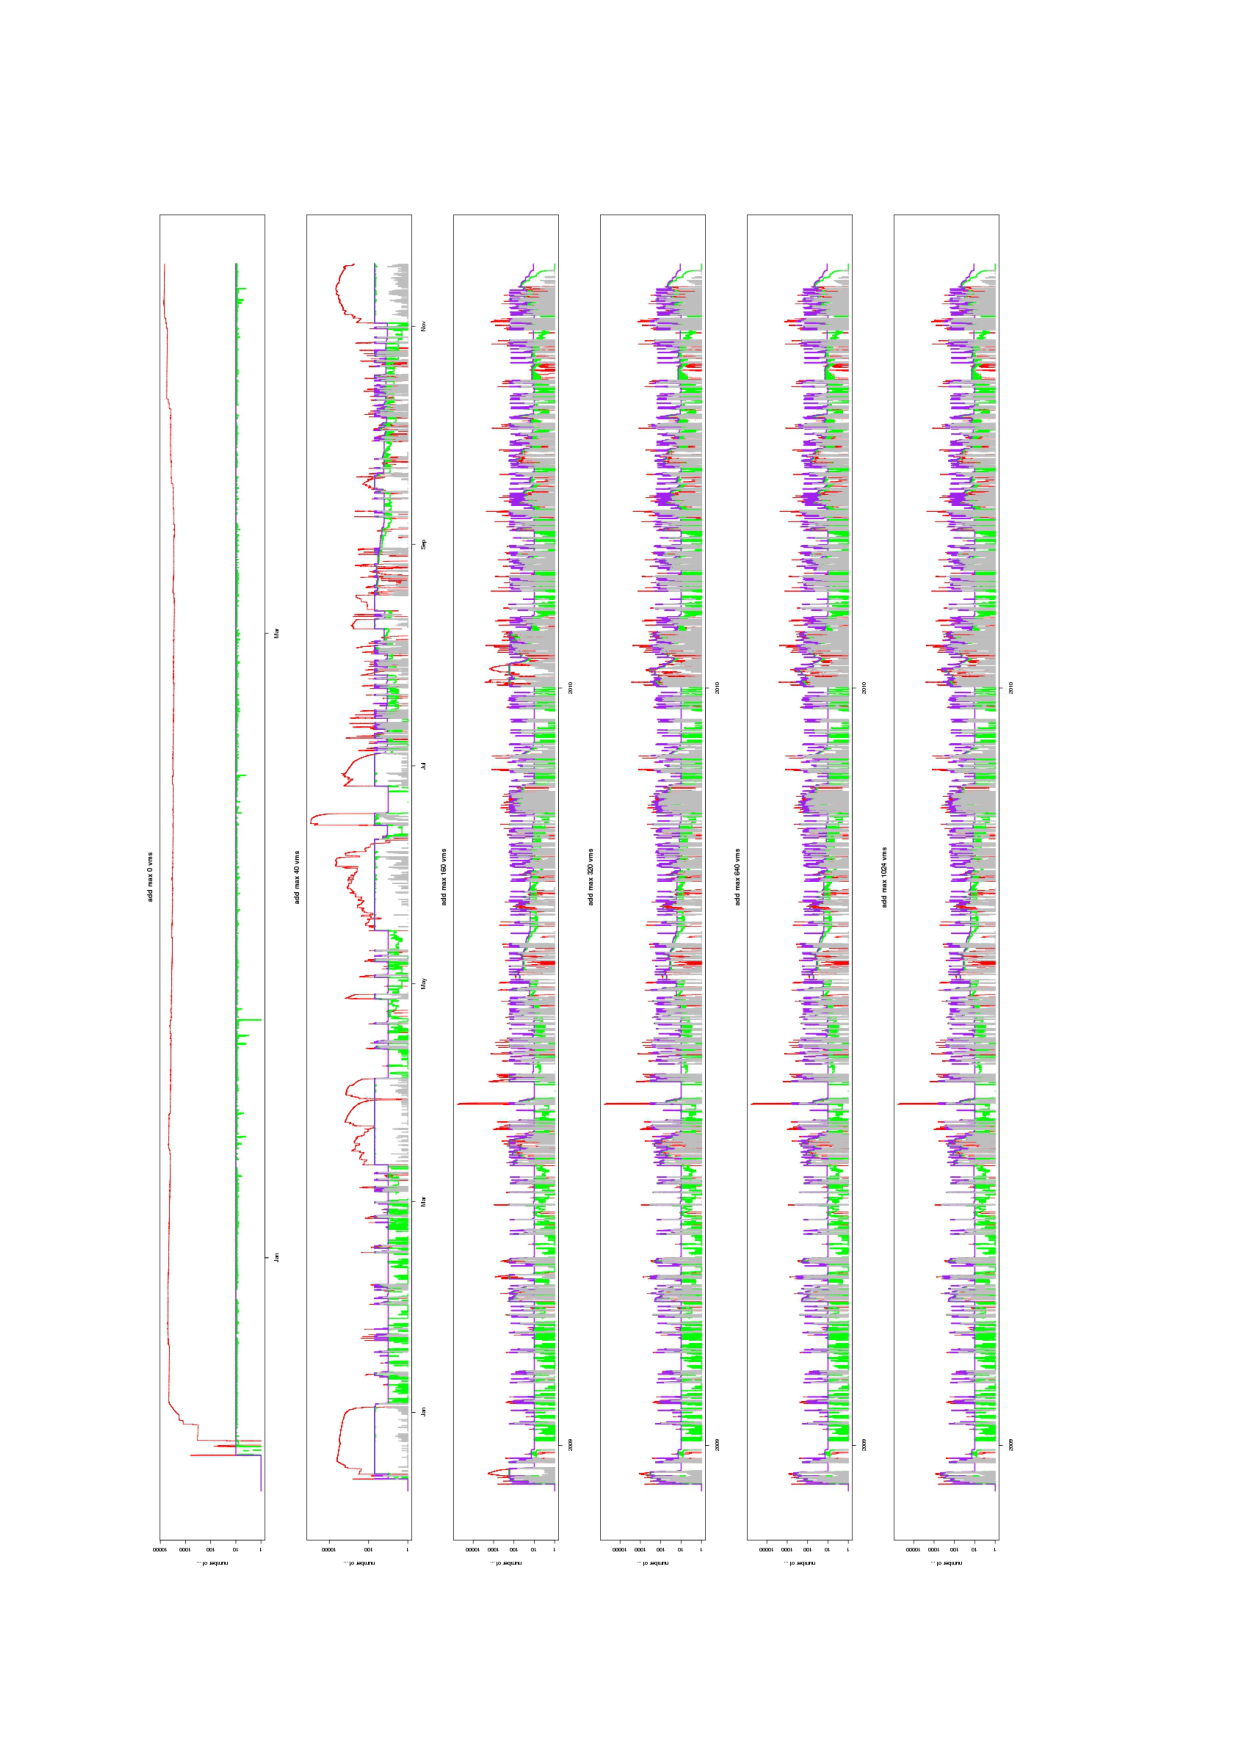
\includegraphics[width=\linewidth,angle=-90,origin=c]{fig/simul}}}
\end{frame}


\begin{frame}[fragile]
  \frametitle{Interface to the cloud(s)}

  \begin{center}
    \href{}{Apache Libcloud} is Python adapter library that abstracts
    away differences among multiple cloud provider APIs.

    \+
    \begin{lstlisting}
def start_vm(self, vm):
  vm.instance = self.provider.create_node(
    name=str(vm.vmid), 
    image=self._images[self.image], 
    size=self._kinds[self.kind])
  ~\em [\ldots]~
    \end{lstlisting}
    \+ 
    Providers exist for EC2, Rackspace, CloudSigma, GoGrid,
    OpenStack, Eucalyptus, \ldots \\
    \href{http://libcloud.apache.org/supported_providers.html}{(more
      than 26 different providers)}
  \end{center}
\end{frame}


\begin{frame}[label=UML]
  \frametitle{Integration with SMSCG / 1}
  \begin{center}
    \href{http://user-mode-linux.sf.net}{User-mode Linux} 
    is a Linux virtualization technology, running entirely in user-space.

    \+
    UML consists of a modified Linux kernel (guest), \\
    that runs as a regular process \\ within another Linux system (host).
  \end{center}
\end{frame}


\begin{frame}
  \frametitle{UML features}
  \label{sec:7}
  Any file in the host system can be a block device (\emph{ubdX}).
  Uses \emph{copy-on-write}, so one filesystem image can be used by many
  UML instances concurrently.

  \+
  Can mount any directory in the host filesystem as a local
  \emph{hostfs} filesystem.
  
  \+
  Outbound net connectivity with a helper program (\emph{slirp}).
  
  \+
  Local networks of UML instances, backing on IP multicast.
\end{frame}


\begin{frame}[label=smscg2]
  \frametitle{Integration with SMSCG / 2}
  \begin{center}
    Idea: \\ \textbf{run a UML machine as a Grid job\textsuperscript{\dag}}

    \+ 
    This allows us to run a ``virtual compute node'' inside the
    compute node of another cluster.

    \+ 
    All we need is a different backend for the Orchestrator, all
    the rest stays the same.

    \+\+
    {\scriptsize \textsuperscript{\dag}: 
      This idea can be taken much further and has spun off into \\
      a software project of its own, named \hyperlink{AppPot}{AppPot}.}
  \end{center}
\end{frame}


\begin{frame}
\begin{center}
  {\Huge Questions ?}

  \+\+
  {\large \bf Thank you!}
\end{center}
\end{frame}


\begin{frame}
  \frametitle{References}
  \begin{center}
    VM-MAD software home: \\ \url{http://vm-mad.googlecode.com}

    \+
    mailing list: \\ \url{virtualization@gc3.lists.uzh.ch}

    \+\+
    {\large \bf Thank you!}
  \end{center}
\end{frame}


\begin{frame}[label=webapp]
  \frametitle{Web frontend screenshot}
  \begin{center}
    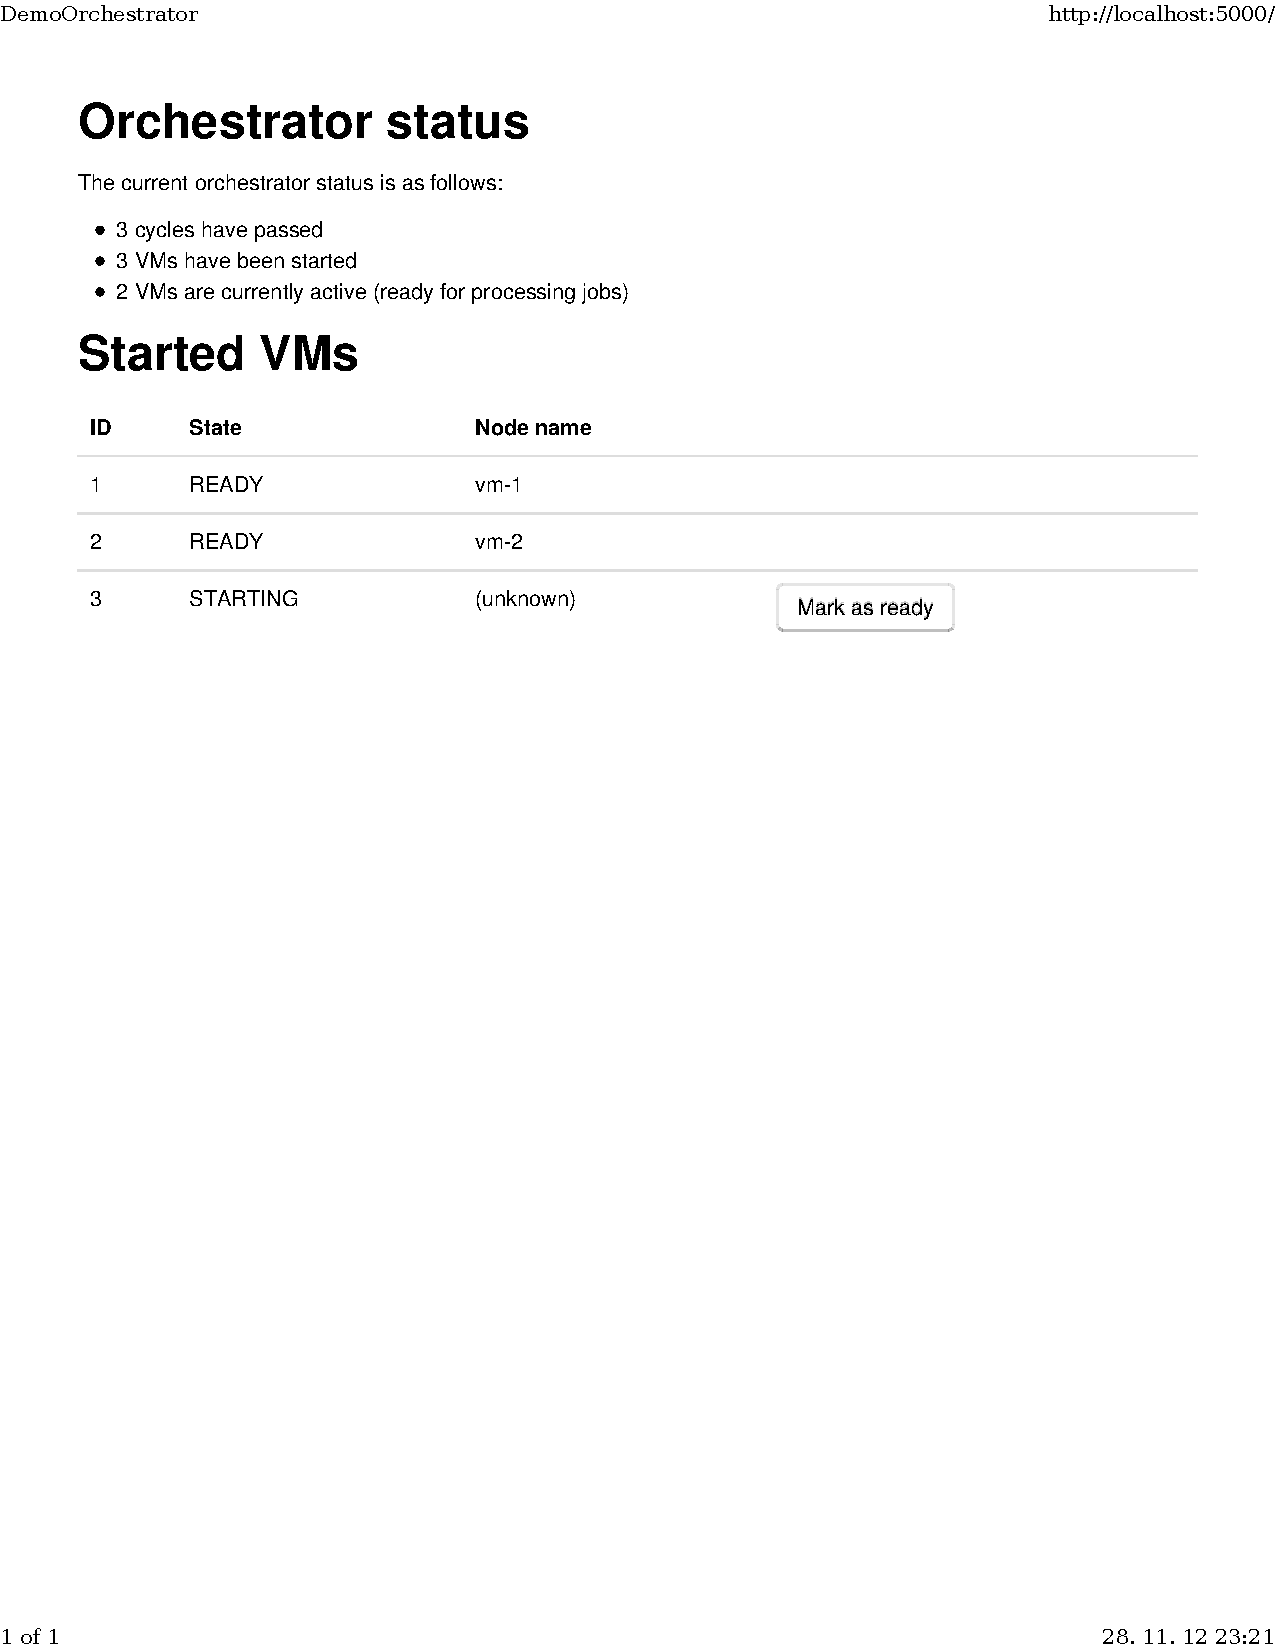
\includegraphics[width=\linewidth]{fig/webapp}
  \end{center}

  \+
  \begin{flushright}
    \hyperlink{features}{\beamergotobutton{Back to main talk}}
  \end{flushright}
\end{frame}


\begin{frame}[label=AppPot]
  \frametitle{AppPot / 1}
  \label{sec:9}
  AppPot consists of:
  \begin{itemize}
  \item a base image (with the AppPot boot script)
    \begin{itemize}
    \item \emph{raw} disk image
    \item can be run in \emph{any} virtualization software: KVM, Xen,
      VirtualBox (and obviously UML!)
    \end{itemize}
  \item a startup script \texttt{apppot-start}
  \item three support programs \texttt{linux}, \texttt{slirp}, \texttt{empty}
  \end{itemize}

  \+
  You can run an AppPot UML machine either locally on your computer,
  textbf{on the Grid}, or in a IaaS cloud.

  \+
  \begin{flushright}
    \hyperlink{smscg2}{\beamergotobutton{Back to main talk}}
  \end{flushright}
\end{frame}


\begin{frame}
  \frametitle{AppPot / 2}
  \label{sec:15}
  AppPot supports a \emph{base} + \emph{changes} mechanism.

  \+
  The command ``\texttt{apppot-snap base}'' records a snapshot of the current
  system state (file sizes, timestamps, etc.).  This should be used by
  sysadmins / application experts when they are done preparing the
  base filesystem image.

  \+
  The command ``\texttt{apppot-snap changes}'' creates a tarball with all the
  modifications since the last recorded base.

  \+
  Users only submit the changes, the startup script automatically
  merges them into the running AppPot instance.

  \+
  \begin{flushright}
    \hyperlink{smscg2}{\beamergotobutton{Back to main talk}}
  \end{flushright}
\end{frame}


\begin{frame}
  \frametitle{AppPot / 3}
  
  \emph{\ldots Complex application deployment?}
  \begin{itemize}
  \item An application expert creates an AppPot base image with the
    software correctly installed and validated.
  \item Users just submit it as a Grid job.
  \end{itemize}

  \+
  \emph{\ldots Running own code on the Grid?}
  \begin{itemize}
  \item  Users get a copy of the base image, install their code in it and do
    the development work (e.g., on their laptops).
  \item  When they want to do a production run, they submit a job attaching the \emph{changes} file.
  \end{itemize}

  \+
  \begin{flushright}
    \hyperlink{smscg2}{\beamergotobutton{Back to main talk}}
  \end{flushright}
\end{frame}

\end{document}
